\documentclass{beamer}

\mode<presentation> {


\usetheme{default}
% \setbeamertemplate{footline} % To remove the footer line in all slides uncomment this line
\setbeamertemplate{footline}[page number] % To replace the footer line in all slides with a simple slide count uncomment this line
\setbeamertemplate{navigation symbols}{} % To remove the navigation symbols from the bottom of all slides uncomment this line
}

\usepackage{graphicx} % Allows including images
\usepackage{booktabs} % Allows the use of \toprule, \midrule and \bottomrule in tables
\usepackage{verbatim}
\usepackage{multicol}

\title[VE215 RC5]{VE215 RC5}
\author{Erdao Liang, Chongye Yang}
\institute[UM-SJTU JI] 
{UM-SJTU JI}
\date{\today}

\begin{document}

\AtBeginSection[ ]
{
\begin{frame}{Overview}
    \tableofcontents[sectionstyle=show/shaded,subsectionstyle=show/shaded/hide]
    % \tableofcontents[sectionstyle=show/shaded,subsectionstyle=show/shaded]
 \end{frame}
}

%%%%%%%%%%%%%%%%%%%%%%%%%%%%%%%%%%%%%%%%%%%%%%%%%%%
% TITLE PAGE
\begin{frame}
\titlepage % Print the title page as the first slide
\end{frame}


%%%%%%%%%%%%%%%%%%%%%%%%%%%%%%%%%%%%%%%%%%%%%%%%%%%
% AC Power Analysis

\section{AC Power Analysis}

%%%%%%%%%%%%%%%%%%%%%%%%%%%%%
\subsection{Instantaneous Power}
\begin{frame}{Instantaneous and Average Power}
Both $v(t)$ and $i(t)$ here are instantaneous values. \textcolor[rgb]{1,0,0}{(not rms)}
$$p(t)=v(t) \cdot i(t)$$
Instantaneous power:
\begin{equation*}
\begin{aligned}
p(t) &= V_{m}I_{m}cos(\omega t + \theta_{v})cos(\omega t + \theta_{i})\\
&= \dfrac{1}{2}V_{m}I_{m}cos(\theta_{v}-\theta_{i})+\dfrac{1}{2}V_{m}I_{m}cos(2 \omega t + \theta_{v} + \theta_{i})
\end{aligned}
\end{equation*}

\end{frame}

%%%%%%%%%%%%%%%%%%%%%%%%%%%%%

\begin{frame}{Average Power}

General definition:
$$P = \frac{1}{T}\int_0^Tp(t)dt$$
For sinusoids,
$$P=\dfrac{1}{2}V_{m}I_{m} cos(\theta_{v}-\theta_{i})$$
Represented with phasor $\tilde{V}$ and $\tilde{I}$,
$$P = \frac12\mathrm{Re}(\tilde{V}\tilde{I^{\color{red}*\color{black}}})$$

\end{frame}

%%%%%%%%%%%%%%%%%%%%%%%%%%%%%
\begin{frame}{Average Power}

\begin{itemize}
    \item when $\theta_{v}-\theta_{i}=0$, purely resistive load $R$.
    $$P = \frac12I_m^2R=\frac12\frac{V_m^2}{R}$$
    (the second equality not true when $\theta_{v}-\theta_{i}\neq 0$)
    
    \item when $\lvert \theta_{v}-\theta_{i} \rvert = 90^{\circ}$, purely reactive load $X$. It absorbs no \textcolor[rgb]{1,0,0}{average} power.
    \item Generally,
    $$\begin{aligned}
        P &= \dfrac{1}{2}V_{m}I_{m} cos(\theta_{v}-\theta_{i}) = \dfrac{1}{2}\mathrm{Re}(\tilde{V} \tilde{I}^{*})= \dfrac{1}{2} \mathrm{Re}((\tilde{I}Z)\tilde{I}^{*})\\
        & = \frac12\mathrm{Re}(I^2R+jI^2X)= \color{red}\dfrac{1}{2} I_{m}^{2}R
    \end{aligned}$$
    (Only resistance contributes to the average power absorbance)
\end{itemize}

\end{frame}

%%%%%%%%%%%%%%%%%%%%%%%%%%%%%
\subsection{Maximum Average Power Transfer}

\begin{frame}{Maximum Average Power Transfer}
\begin{figure}
\centering
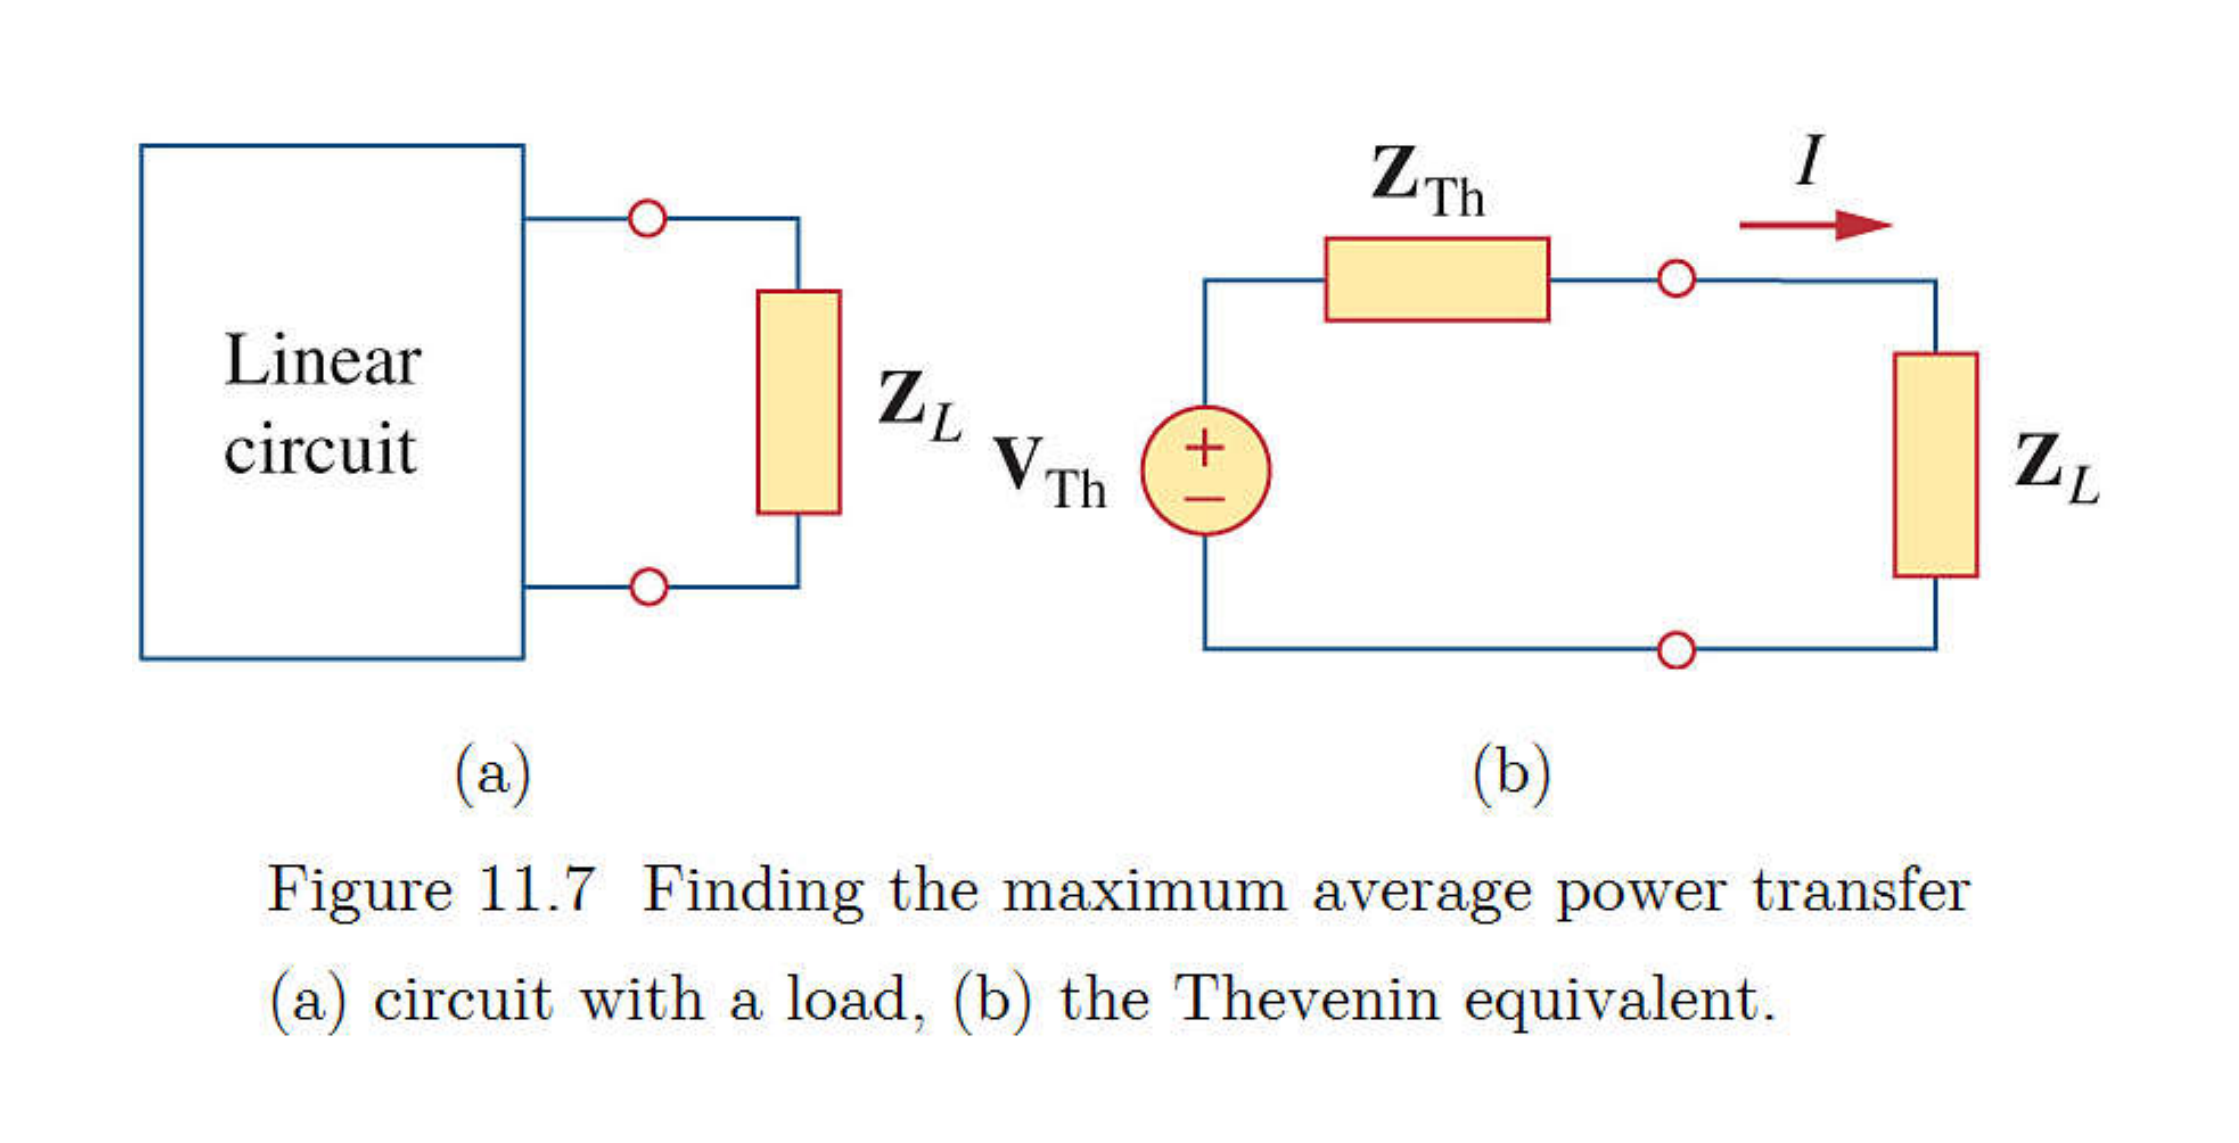
\includegraphics[width=3.5in]{img_ch11/maximum_power.png}
\end{figure}
\begin{itemize}
\item If there is no restriction on $Z_L$,
$$R_{L}=R_{Th}\ \ \ X_{L}=-X_{Th}\ \ \ P_{max}=\dfrac{\lvert V_{Th }^{2} \rvert}{8R_{Th}}$$
\item If $Z_L$ is purely resistive,
$$R_{L}=\sqrt{R_{Th}^{2}+X_{Th}^{2}}$$
\end{itemize}
\end{frame}

%%%%%%%%%%%%%%%%%%%%%%%%%%%%%
\subsection{Effective or RMS Value}
% TODO: motivation and definition
% TODO:重新排版
\begin{frame}{Effective or RMS Value}

Definition: The effective value of a periodic current is the dc current that delivers the same average power to a resistor as the periodic current (similarly for voltage).
$$I_{eff}^2R = \frac{R}{T}\int_0^Ti^2dt$$

Effective value = RMS (root mean square) value.


\begin{equation*}
\begin{aligned}
I_{rms} &= \sqrt{\dfrac{1}{T} \int_{0}^{T} i^{2} \mathrm{d} t} = I_{eff} \\
V_{rms} &= \sqrt{\dfrac{1}{T} \int_{0}^{T} v^{2} \mathrm{d} t} = V_{eff} \\
\end{aligned}
\end{equation*}

\end{frame}

%%%%%%%%%%%%%%%%%%%%%%%%%%%%%

\begin{frame}{Effective or RMS Value}

\begin{itemize}
    \item Avg power absorbed by a circuit element (generally true):
$$P = I_{rms}^R=V_{rms}^2\frac{R}{R^2+X^2}$$
\begin{tiny}
\begin{center}
    $P = \dfrac{1}{2}\mathrm{Re}(\tilde{V}\tilde{I}^{*})=\mathrm{Re}(\tilde{V_{rms}}\tilde{I^{*}_{rms}}) = \dfrac{1}{2} I_{m}^{2} R=I_{rms}^{2}R = \dfrac{1}{2} V_{m}^{2} \mathrm{Re} (\dfrac{1}{Z^{*}}) = V_{rms}^{2} \dfrac{R}{R^{2}+X^{2}}$
\end{center}

\hspace{0.1mm}
\end{tiny}
    \item RMS value for a sinusoid \color{red} sinusoid\color{black}: 
\begin{equation*}
I_{rms} = \dfrac{I_{m}}{\sqrt{2}} \qquad
V_{rms} = \dfrac{V_{m}}{\sqrt{2}}
\end{equation*}

    \item Average power absorbed by an element in a \color{red}sinusoidal \color{black}  circuit:

    $$P = V_{rms}I_{rms}\cos(\theta_v-\theta_i)$$
    
\end{itemize}

\end{frame}

\begin{frame}{Effective or RMS Value}

\textbf{Caution: from now on, unless specified, all values will be assumed to be RMS values.}
\end{frame}

%%%%%%%%%%%%%%%%%%%%%%%%%%%%%

\subsection{Complex Power}
\begin{frame}{Complex Power}

We define this ``complex power" that includes all the information.

$$\begin{aligned}
    \text{Complex Power}&=\tilde{S}=\tilde{V_{rms}}\tilde{I_{rms}^{\color{red}*\color{black}}} = \lvert I_{rms}\rvert \lvert V_{rms} \rvert \angle (\theta_{v}\color{red}-\color{black}\theta_{i})\\
    &=\lvert S \rvert \angle (\theta_{v}\color{red}-\color{black}\theta_{i}) \text{ (polar form)}\\
    &= P+jQ \text{ (rectangular form)}
\end{aligned}$$

\begin{table}[]
    \centering
    \begin{tabular}{cccc}
        \toprule
        Value & Name & Meaning & Unit \\
        \midrule
        $\vert S\vert$ & Apparent power & Magnitude of $\tilde{S}$ & VA \\
        $\cos(\theta_v-\theta_i)$ & Power factor & Cosine of angle of $\tilde{S}$  & / \\ 
        $P$ & Real power & Real part of $\tilde{S}$ & W \\
        $Q$ & Complex power & Imaginary part of $\tilde{S}$ & VAR  \\
        \bottomrule
    \end{tabular}
\end{table}


\end{frame}

%%%%%%%%%%%%%%%%%%%%%%%%%%%%%
\begin{frame}{Complex Power}

\begin{itemize}
    \item Complex power
    \begin{center}
        $
        \tilde{S}=\tilde{V_{rms}}\tilde{I_{rms}^{\color{red}*\color{black}}} = \lvert I_{rms}\rvert \lvert V_{rms} \rvert \angle (\theta_{v}\color{red}-\color{black}\theta_{i}) =\lvert S \rvert \angle (\theta_{v}\color{red}-\color{black}\theta_{i}) = P+jQ
        $
        \hspace{0.1mm}
        $
        \tilde{S} = {\vert I_{rms} \vert}^2Z = \frac{{\vert V_{rms}\vert}^2}{Z^{\color{red}*\color{black}}}
        $
    \end{center}
        
    \item Apparent power
     $$
     \lvert S \rvert=  \vert V_{rms}\vert\vert I_{rms}\vert =\lvert I_{rms} \rvert ^{2} \lvert Z \rvert = \sqrt{P^2+Q^2}
     $$

    \item Real power
    $$P = \mathrm{Re}(\tilde{S}) = \vert S\vert \cos(\theta_v-\theta_i) = \lvert I_{rms} \rvert ^{2} R$$
    \item Complex power
    $$Q = \mathrm{Im}(\tilde{S}) = \vert S\vert \sin(\theta_v-\theta_i) = \lvert I_{rms} \rvert ^{2} X$$
    \item Power factor
    $$
    \text{pf} = \frac{P}{\vert S\vert} = \cos(\theta_v-\theta_i)
    $$
\end{itemize}

\end{frame}

\begin{frame}{Complex Power}
    Power factor
    $
    \text{pf} = \frac{P}{\vert S\vert} = \cos(\theta_v-\theta_i)
    $:
    \begin{itemize}
        \item $\theta_v - \theta_i < 0$: leading pf
        \item $\theta_v - \theta_i >0$: lagging pf
    \end{itemize}
    
    Since $\cos (\theta_v - \theta_i) = \cos (\theta_i - \theta_v)$, the pf value only tells part of the story. Every time you are asked for a power factor, \color{red} you must declare whether it is leading or lagging\color{black}.
\end{frame}

%%%%%%%%%%%%%%%%%%%%%%%%%%%%%

\begin{frame}{Complex Power}

We can use the sign of pf angle or $Q$ to identify the property of the circuit and the loads:

\begin{table}[]
    \centering
    \begin{tabular}{c|c|c|c}
        \hline
        &(1)&(2)&(3)\\
        \hline
        pf Angle & $\theta_v-\theta_i=0$ & $\theta_v-\theta_i<0$ & $\theta_v-\theta_i>0$  \\ 
        Sign of $Q$ &$Q = 0$ & $Q<0$ & $Q>0$ \\
        \hline
        &Unity pf & Leading pf & Lagging pf \\
        Properties &$I$, $V$ in phase & $I$ leads $V$ & $I$ lags $V$ \\
        &$X = 0$ & $X<0$& $X>0$\\
        &Resistive loads&Capacitive loads&Inductive loads\\
        \hline
        
    \end{tabular}
\end{table}
    
\end{frame}

%%%%%%%%%%%%%%%%%%%%%%%%%%%%%
\begin{frame}{Complex Power}

\begin{multicols}{2}
        \sectiont{}
\begin{figure}
    \centering
    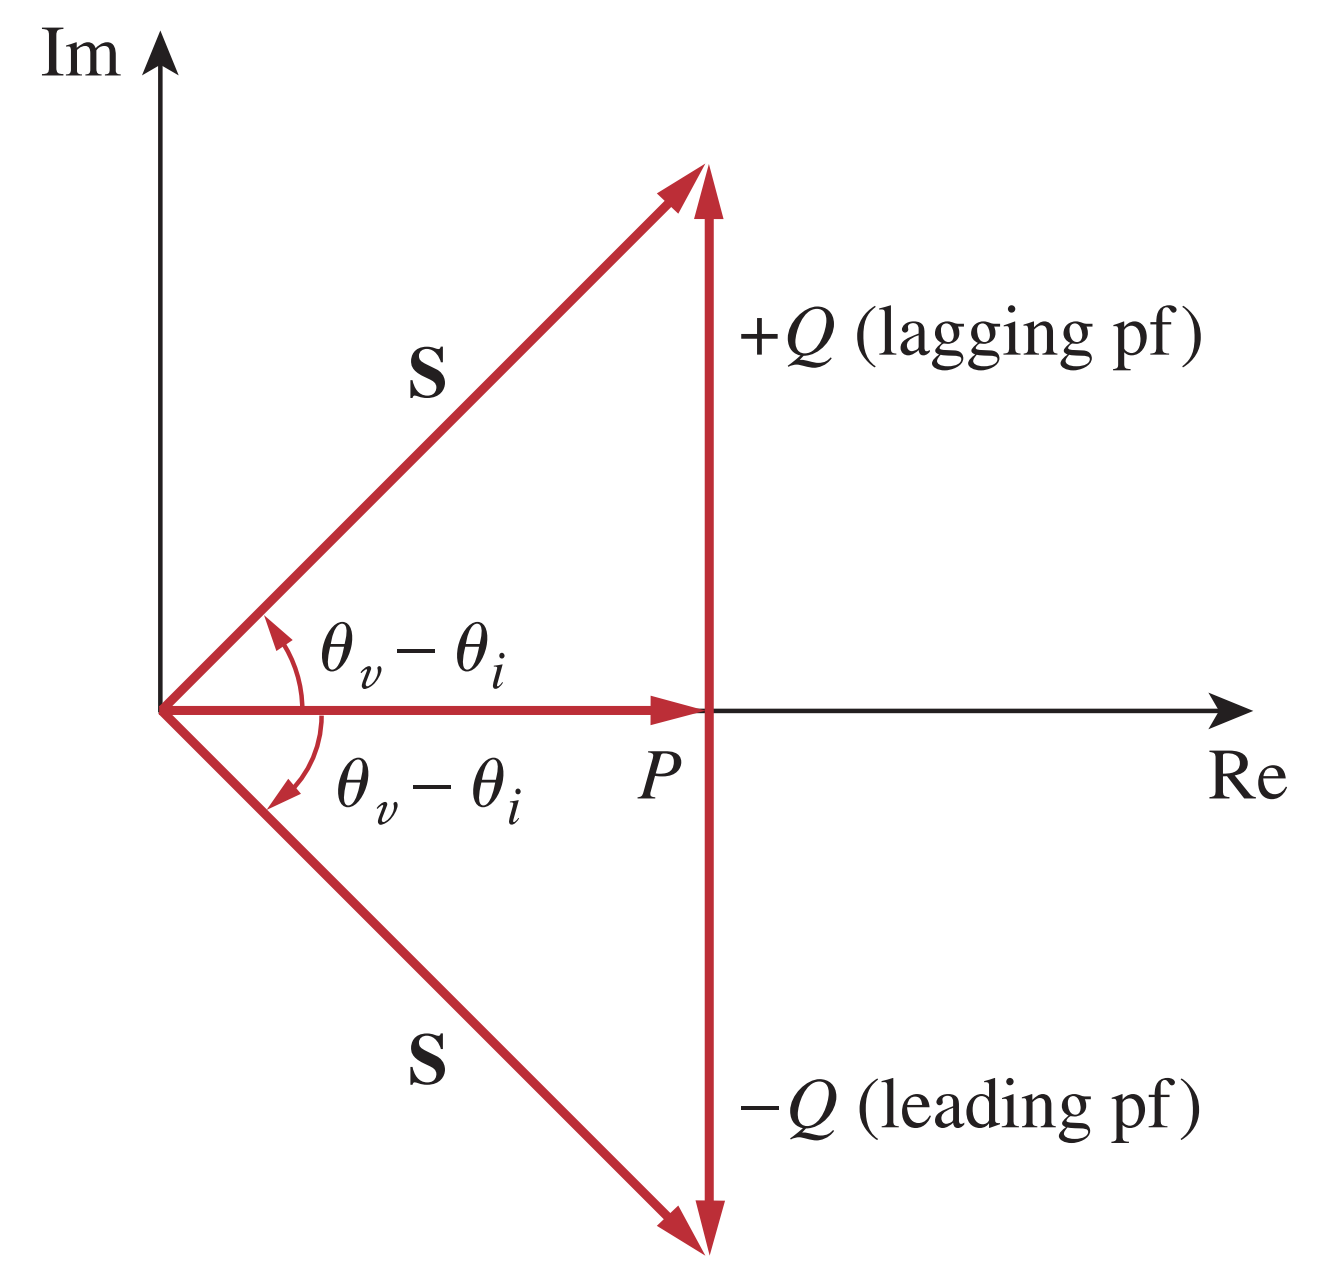
\includegraphics[width=0.48\textwidth]{img_ch11/power triangle.png}
\end{figure}
        \sectiont{}
And observe that the power factor angle is equal to the angle of the impedance of that part of the circuit.
\begin{figure}
\centering
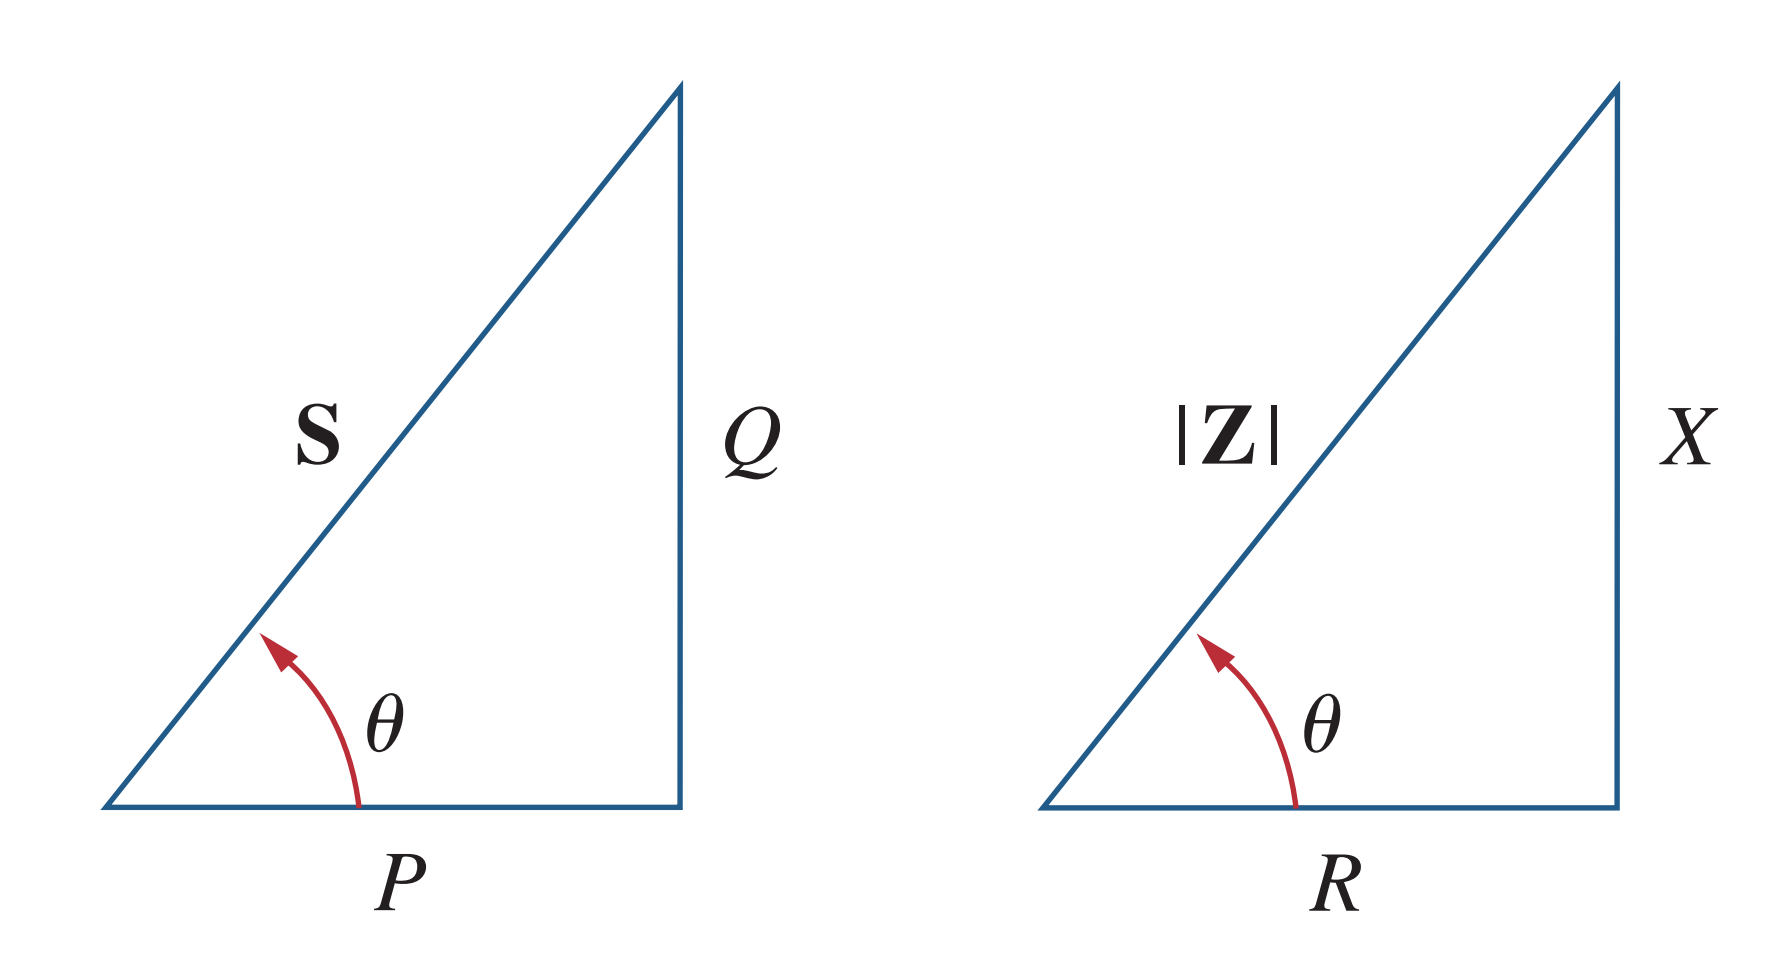
\includegraphics[width=0.48\textwidth]{img_ch11/pf.png}
\end{figure}
        
        
\end{multicols}
\end{frame}



%%%%%%%%%%%%%%%%%%%%%%%%%%%%%
\begin{frame}{Exercise 1}
\textbf{Question}:
\newline
A series-connected load draws a current $i(t)=4cos(100\pi t+10^{\circ}) A$ when the applied voltage is $v(t)=120cos(100\pi t-20^{\circ})V$. Find the apparent power and the power factor of the load. Determine the element values that form the series-connected load.
\end{frame}

%%%%%%%%%%%%%%%%%%%%%%%%%%%%%
\begin{frame}{Exercise 1}
\begin{figure}
\centering
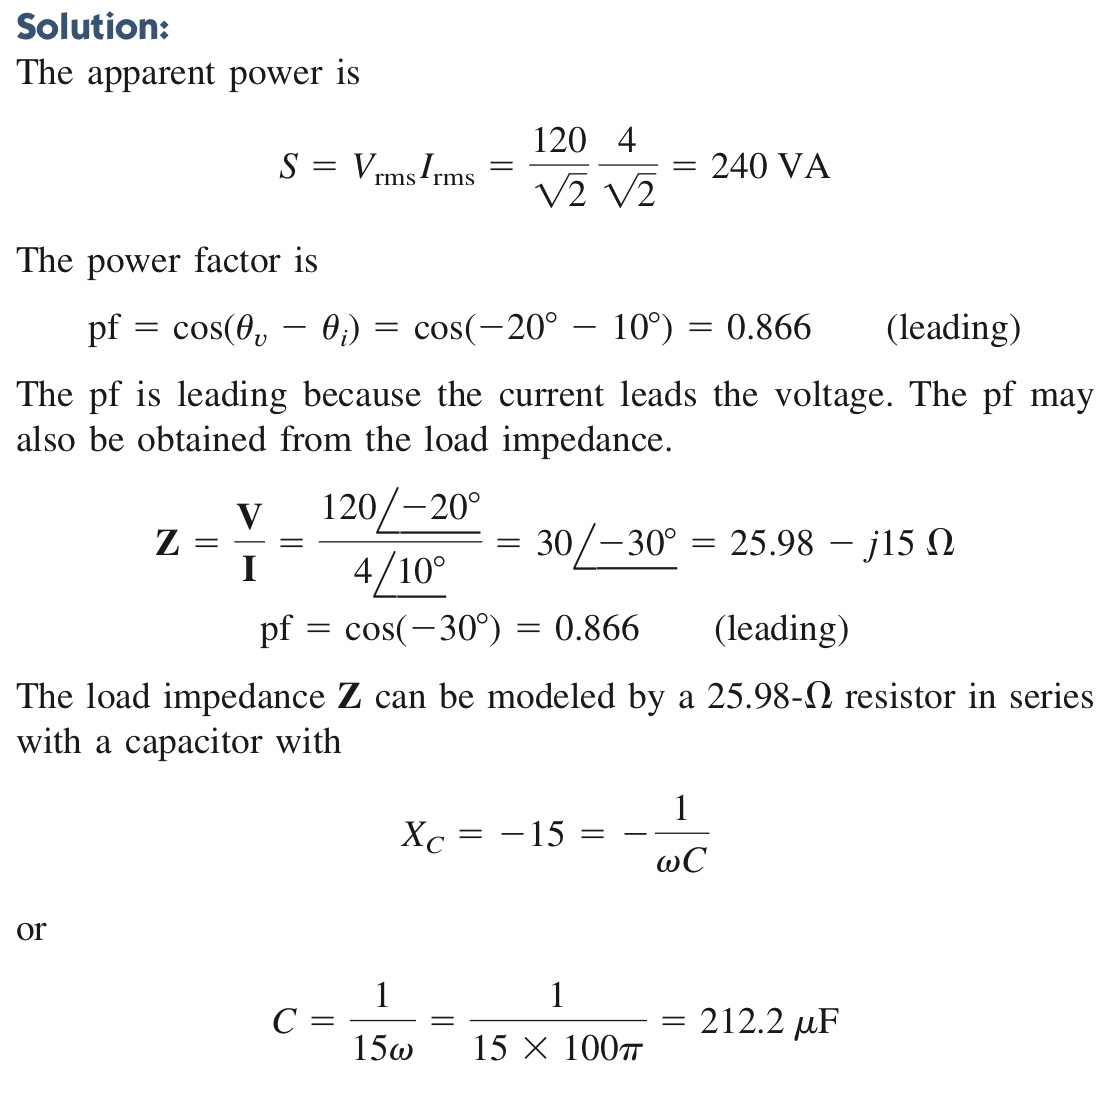
\includegraphics[width=3in]{img_ch11/s1.jpg}
\end{figure}  
\end{frame}

%%%%%%%%%%%%%%%%%%%%%%%%%%%%%
\subsection{Power Factor Correction}

\begin{frame}{Power Factor Correction}
\begin{itemize}
    \item Goal: increase the pf of a load $\rightarrow$ make it less inductive $\rightarrow$ reduce energy loss

    \item Solution: add a capacitor in parallel to the load

    \begin{figure}
        \centering
        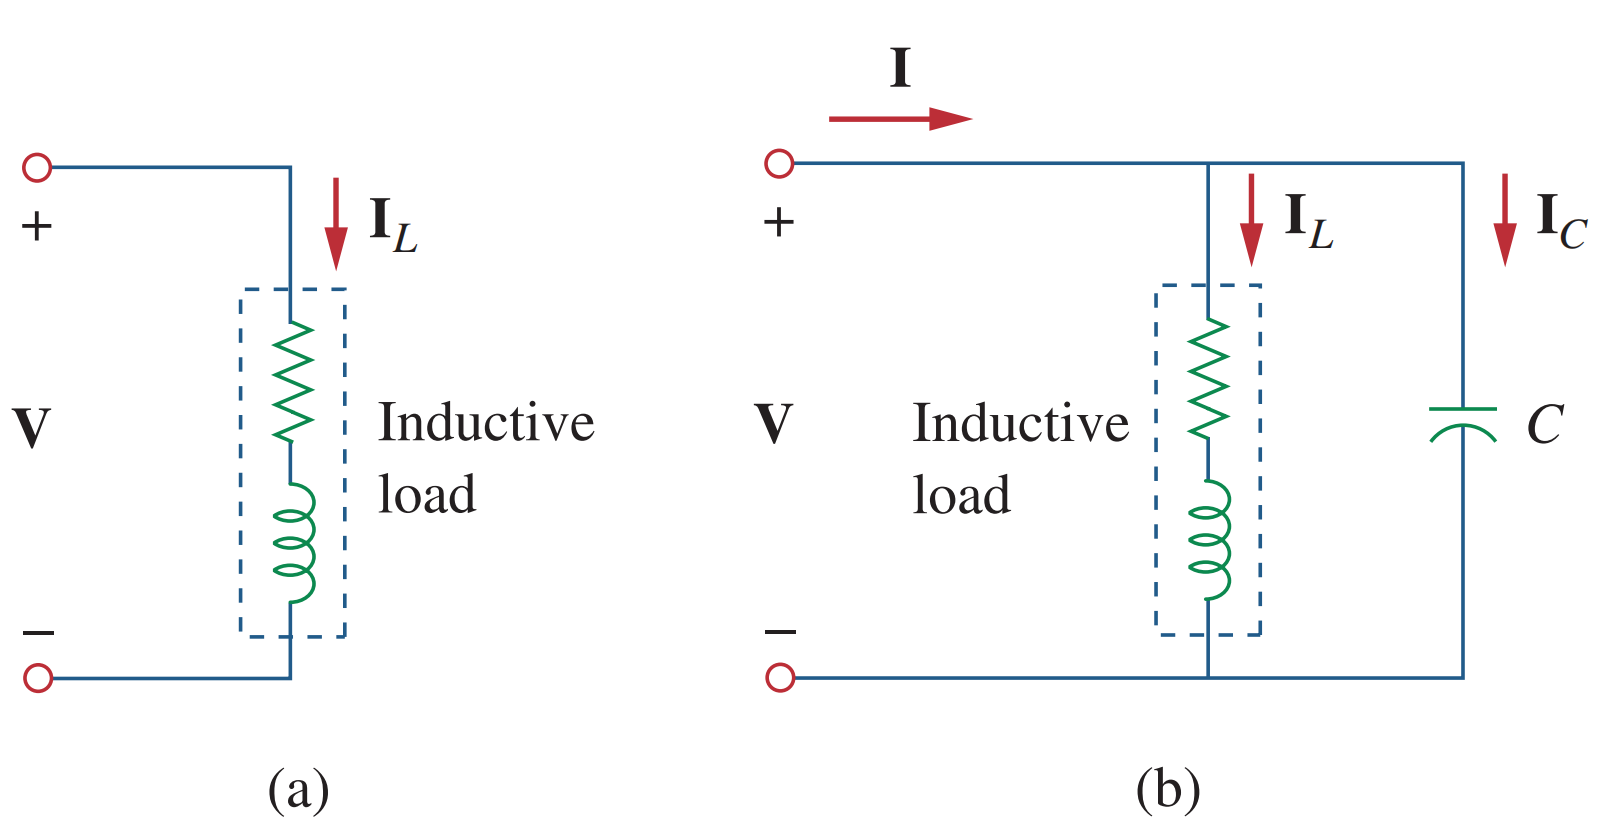
\includegraphics[width=0.7\textwidth]{img_ch11/add capacitor.png}
    \end{figure}
    
\end{itemize}

\end{frame}

%%%%%%%%%%%%%%%%%%%%%%%%%%%%%
\begin{frame}{Power Factor Correction}

Goal: increase the pf from $\cos \theta_1$ to $\cos \theta_2$.
\begin{multicols}{2}
\sectiont{}
\begin{figure}
    \centering
    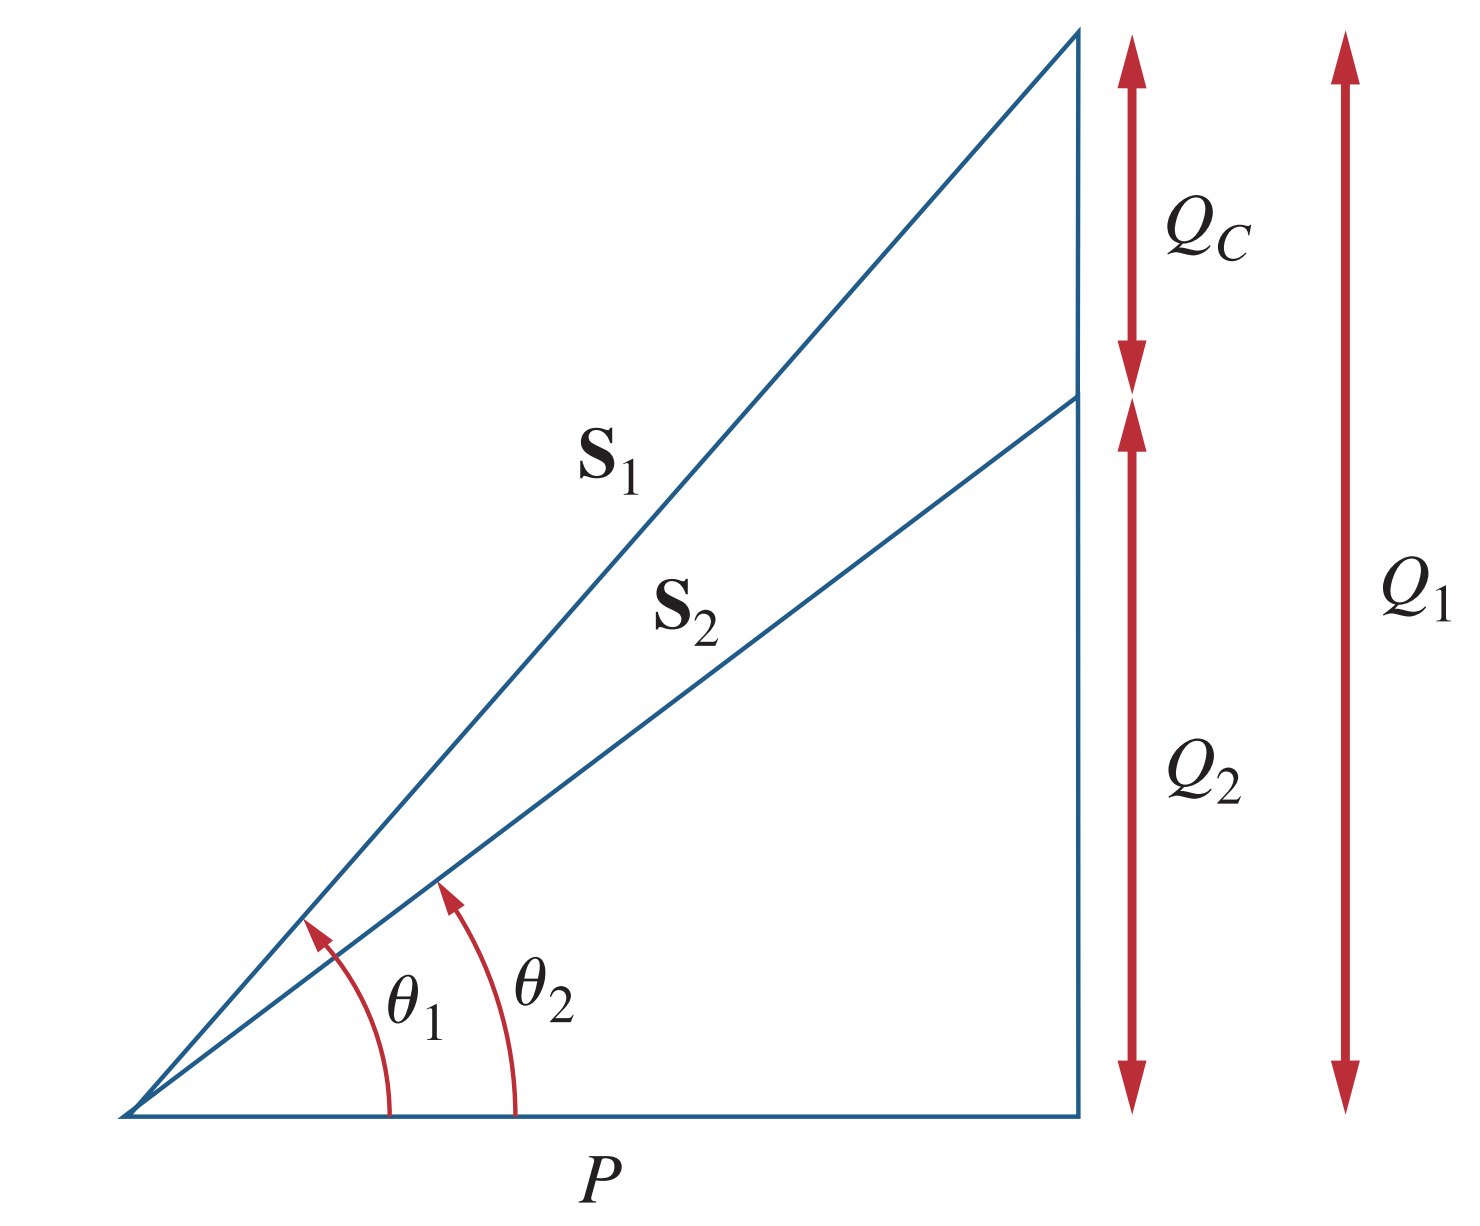
\includegraphics[width=0.4\textwidth]{img_ch11/triangle2.png}
\end{figure}
\sectiont{}
Initial:

$P = \vert S_1\vert \cos \theta_1$

$Q_1 = \vert Q_1\vert \sin \theta_1= P \tan \theta_1$

\vspace{0.3cm}
The ``after" we expect:

$P = \vert S_2\vert \cos \theta_2$

$Q_2 = \vert Q_2\vert \sin \theta_2= P \tan \theta_2$
        
\end{multicols}

Since $Q_c(=Q_1-Q_2)= \frac{V_{rms}^2}{X_c}$, then the value of the required capacitance $C$ is 
$$C = \frac{Q_C}{\omega V_{rms}^2} = \frac{Q_2-Q_1}{\omega V_{rms}^2} = \color{red}\frac{P(\tan \theta_1 - \tan \theta_2)}{\omega V_{rms}^2}$$
\end{frame}


%%%%%%%%%%%%%%%%%%%%%%%%%%%%%
\begin{frame}{Exercise 2}
\textbf{Question}:
\newline
When connected to a 120-V (rms), 60-Hz power line, a load absorbs 4 kW at a lagging power factor of 0.8. Find the value of capacitance necessary to raise the pf to 0.95.
\end{frame}

%%%%%%%%%%%%%%%%%%%%%%%%%%%%%
\begin{frame}{Exercise 2}
\textbf{Question}:
\newline
When connected to a 120-V (rms), 60-Hz power line, a load absorbs 4 kW at a lagging power factor of 0.8. Find the value of capacitance necessary to raise the pf to 0.95.
\newline
\newline
\textbf{Formula}: $C=\dfrac{P  \tan(\theta_{1}-\theta_{2})}{\omega \cdot V_{rms}^{2}}$
\newline
\newline
\textbf{Answer}: 310.5 $\mu$F
\end{frame}

%%%%%%%%%%%%%%%%%%%%%%%%%%%%%%%%%%%%%%%%%%%%%%%%%%%
% Three Phase Circuit

% \section{Three-Phase Circuits}




%%%%%%%%%%%%%%%%%%%%%%%%%%%%%%%%%%%%%%%%%%%%%%%%%%%
\begin{frame}
\frametitle{References}
\begin{enumerate}
\item 2023 Summer VE215 slides, Rui Yang
\item Fundamentals of Electric Circuits, 5th e, Sadiku, Matthew
\item 2022 Fall RC5, Yuxuan Peng
\item 2022 Fall RC6, Zhiyu Zhou
\end{enumerate}
\end{frame}


\begin{frame}
\Huge{\centerline{Thank you!}}
\end{frame}


\end{document}
